\problema{6}{Difusión 2D estacionaria}{7}

\begin{enunciado}
	Sea $-D\nabla^2\varphi + \Sigma_a\varphi = S$ en un cuadrado con $\varphi = 0$ en la frontera y una
	malla uniforme con $h = L/3$ (cuatro nodos interiores numerados en orden lexicográfico).
	Tome $D/h^2 = 1$, $\Sigma_a = 0$ y $S = 1$.
	
	\begin{center}
		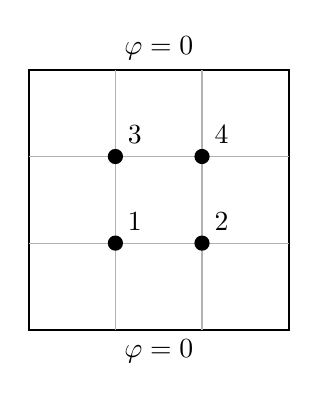
\begin{tikzpicture}[scale=1.1]
			\draw[thick] (0,0) rectangle (3,3);
			\draw[gray!60] (1,0) -- (1,3) (2,0) -- (2,3) (0,1) -- (3,1) (0,2) -- (3,2);
			\foreach \x/\y/\n in {1/1/1, 2/1/2, 1/2/3, 2/2/4} {
				\fill (\x,\y) circle (2.5pt);
				\node[above right=1pt] at (\x,\y) {$\n$};
			}
			\node[below] at (1.5,0) {$\varphi = 0$};
			\node[above] at (1.5,3) {$\varphi = 0$};
		\end{tikzpicture}
	\end{center}
	
	\begin{enumerate}[label=(\alph*)]
		\item Deduzca el esquema de cinco puntos y muestre que su error de truncamiento es $\Order{h^2}$.
		\item Ensamble $\mat{A}\vect{\varphi} = \vect{b}$ y señale la estructura por bloques.
		\item Calcule el factor de Cholesky $\mat{G}$ de $\mat{A}$.
		\item Resuelva el sistema con $\mat{G}$.
		\item Para una malla de $n\times n$ nodos interiores, indique el tamaño de $\mat{A}$, su
		semiancho de banda y explique el \emph{relleno} (\emph{fill-in}) que produce la factorización.
	\end{enumerate}
\end{enunciado}

\[
-D\,\frac{\partial^2 \varphi}{\partial x^2} - D\,\frac{\partial^2 \varphi}{\partial y^2} + \Sigma_a\,\varphi(x,y) = S,
\qquad \varphi = 0 \ \text{en la frontera},
\qquad \frac{D}{h_x^2} = \frac{D}{h_y^2} = 1 .
\]

\inciso{a}{Esquema de cinco puntos y error de truncamiento}

\paso{1}{Generación del mallado}
Con $I = J = 3$ en cada dirección:
\[
x_i = i\,h_x, \qquad y_j = j\,h_y, \qquad i, j = 0, 1, 2, 3 .
\]
Los nodos con $i$ o $j$ igual a $0$ o $3$ están en la frontera $\varphi = 0$ y quedan $(I-1)(J-1) = 4$ incgnitas

\paso{2}{Colocación de la EDP en el nodo $(x_i, y_j)$}
\[
-D\left.\frac{\partial^2 \varphi}{\partial x^2}\right|_{(x_i,y_j)}
- D\left.\frac{\partial^2 \varphi}{\partial y^2}\right|_{(x_i,y_j)}
+ \Sigma_a\,\varphi(x_i,y_j) = S, \qquad i, j = 1, 2 .
\]

\paso{3}{Cambio de las derivadas por segundas diferencias divididas centradas}
Con Taylor alrededor de $x_i$ con $y_j$ fijo 
\begin{align*}
	\varphi(x_i + h_x, y_j) &= \varphi + h_x \varphi_x + \frac{h_x^2}{2}\varphi_{xx} + \frac{h_x^3}{6}\varphi_{xxx}
	+ \frac{h_x^4}{24}\varphi_{xxxx} + \frac{h_x^5}{120}\varphi_{xxxxx} + \Order{h_x^6}\\
	\varphi(x_i - h_x, y_j) &= \varphi - h_x \varphi_x + \frac{h_x^2}{2}\varphi_{xx} - \frac{h_x^3}{6}\varphi_{xxx}
	+ \frac{h_x^4}{24}\varphi_{xxxx} - \frac{h_x^5}{120}\varphi_{xxxxx} + \Order{h_x^6}
\end{align*}
Al sumar, los términos de orden impar se cancelan 
\begin{align*}
	\varphi(x_i + h_x, y_j) &= \varphi + \bcancel{h_x \varphi_x} + \frac{h_x^2}{2}\varphi_{xx} + \bcancel{\frac{h_x^3}{6}\varphi_{xxx}}
	+ \frac{h_x^4}{24}\varphi_{xxxx} + \bcancel{\frac{h_x^5}{120}\varphi_{xxxxx}} + \Order{h_x^6}\\
	\varphi(x_i - h_x, y_j) &= \varphi - \bcancel{h_x \varphi_x} + \frac{h_x^2}{2}\varphi_{xx} - \bcancel{\frac{h_x^3}{6}\varphi_{xxx}}
	+ \frac{h_x^4}{24}\varphi_{xxxx} - \bcancel{\frac{h_x^5}{120}\varphi_{xxxxx}} + \Order{h_x^6}
\end{align*}
y los pares se duplican
($\frac{h_x^2}{2!} + \frac{h_x^2}{2!} = h_x^2$ y $\frac{h_x^4}{4!} + \frac{h_x^4}{4!} = \frac{h_x^4}{12}$):
\[
\varphi(x_{i+1}, y_j) + \varphi(x_{i-1}, y_j) = 2\varphi(x_i, y_j) + h_x^2 \varphi_{xx} + \frac{h_x^4}{12}\varphi_{xxxx} + \Order{h_x^6}.
\]
Despejando y dividiendo entre $h_x^2$:
\[
\frac{\varphi(x_{i+1}, y_j) - 2\varphi(x_i, y_j) + \varphi(x_{i-1}, y_j)}{h_x^2}
= \left.\frac{\partial^2 \varphi}{\partial x^2}\right|_{(x_i,y_j)} + \frac{h_x^2}{12}\,\varphi_{xxxx} + \Order{h_x^4}
= \varphi_{xx} + \Order{h_x^2}.
\]

Se hace lo mismo $y$, con Taylor alrededor de $y_j$ con $x_i$ fijo y notamos que es el mismo procedimient
\begin{align*}
	\varphi(x_i, y_j + h_y) &= \varphi + h_y \varphi_y + \frac{h_y^2}{2}\varphi_{yy} + \frac{h_y^3}{6}\varphi_{yyy}
	+ \frac{h_y^4}{24}\varphi_{yyyy} + \frac{h_y^5}{120}\varphi_{yyyyy} + \Order{h_y^6}\\
	\varphi(x_i, y_j - h_y) &= \varphi - h_y \varphi_y + \frac{h_y^2}{2}\varphi_{yy} - \frac{h_y^3}{6}\varphi_{yyy}
	+ \frac{h_y^4}{24}\varphi_{yyyy} - \frac{h_y^5}{120}\varphi_{yyyyy} + \Order{h_y^6}
\end{align*}
Al sumar, los términos de orden impar se cancelan
\begin{align*}
	\varphi(x_i, y_j + h_y) &= \varphi + \bcancel{h_y \varphi_y} + \frac{h_y^2}{2}\varphi_{yy} + \bcancel{\frac{h_y^3}{6}\varphi_{yyy}}
	+ \frac{h_y^4}{24}\varphi_{yyyy} + \bcancel{\frac{h_y^5}{120}\varphi_{yyyyy}} + \Order{h_y^6}\\
	\varphi(x_i, y_j - h_y) &= \varphi - \bcancel{h_y \varphi_y} + \frac{h_y^2}{2}\varphi_{yy} - \bcancel{\frac{h_y^3}{6}\varphi_{yyy}}
	+ \frac{h_y^4}{24}\varphi_{yyyy} - \bcancel{\frac{h_y^5}{120}\varphi_{yyyyy}} + \Order{h_y^6}
\end{align*}
y los pares se duplican:
\[
\varphi(x_i, y_{j+1}) + \varphi(x_i, y_{j-1}) = 2\varphi(x_i, y_j) + h_y^2 \varphi_{yy} + \frac{h_y^4}{12}\varphi_{yyyy} + \Order{h_y^6}.
\]
Despejando y dividiendo entre $h_y^2$:
\[
\frac{\varphi(x_i, y_{j+1}) - 2\varphi(x_i, y_j) + \varphi(x_i, y_{j-1})}{h_y^2}
= \left.\frac{\partial^2 \varphi}{\partial y^2}\right|_{(x_i,y_j)} + \frac{h_y^2}{12}\,\varphi_{yyyy} + \Order{h_y^4}
= \varphi_{yy} + \Order{h_y^2}.
\]

Al quitar los terminos de error, se vuelven aproximaciones. Lo introducimos en la EDP original:
\[
-D\,\frac{\varphi_{i+1,j} - 2\varphi_{ij} + \varphi_{i-1,j}}{h_x^2}
- D\,\frac{\varphi_{i,j+1} - 2\varphi_{ij} + \varphi_{i,j-1}}{h_y^2} + \Sigma_a\,\varphi_{ij} = S .
\]
Agrupando los coeficientes de cada nodo:
\resultado{-\frac{D}{h_y^2}\varphi_{i,j-1} - \frac{D}{h_x^2}\varphi_{i-1,j}
	+ \left(\frac{2D}{h_x^2} + \frac{2D}{h_y^2} + \Sigma_a\right)\varphi_{ij}
	- \frac{D}{h_x^2}\varphi_{i+1,j} - \frac{D}{h_y^2}\varphi_{i,j+1} = S}
Con $h_x = h_y = h$ la diagonal queda $\frac{4D}{h^2} + \Sigma_a$.

Con $D/h_x^2 = D/h_y^2 = 1$, $\Sigma_a = 0$ y $S = 1$ queda el "stencil" de cinco puntos
\[
4\varphi_{ij} - \varphi_{i-1,j} - \varphi_{i+1,j} - \varphi_{i,j-1} - \varphi_{i,j+1} = 1, \qquad i, j = 1, 2 .
\]

\begin{center}
	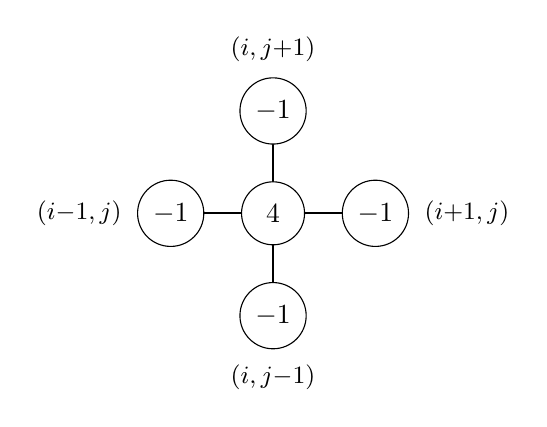
\begin{tikzpicture}[scale=1.3]
		\draw[thick] (-1,0) -- (1,0) (0,-1) -- (0,1);
		\foreach \x/\y/\w in {0/0/4, 1/0/-1, -1/0/-1, 0/1/-1, 0/-1/-1} {
			\node[circle, draw, fill=white, minimum size=8mm] at (\x,\y) {$\w$};
		}
		\node[right=5mm] at (1,0)  {\small $(i{+}1,j)$};
		\node[left=5mm]  at (-1,0) {\small $(i{-}1,j)$};
		\node[above=5mm] at (0,1)  {\small $(i,j{+}1)$};
		\node[below=5mm] at (0,-1) {\small $(i,j{-}1)$};
	\end{tikzpicture}
\end{center}

\paso{4}{Error de truncamiento}
El error de truncamiento es lo que sobra al meter la solución \emph{exacta} en el esquema:
\begin{align*}
\tau_{ij} = &-D\,\frac{\varphi(x_{i+1}, y_j) - 2\varphi(x_i, y_j) + \varphi(x_{i-1}, y_j)}{h_x^2}\\
&- D\,\frac{\varphi(x_i, y_{j+1}) - 2\varphi(x_i, y_j) + \varphi(x_i, y_{j-1})}{h_y^2}
+ \Sigma_a\varphi(x_i, y_j) - S .
\end{align*}
Usando los resultados del paso 3:
\[
\tau_{ij} = -D\left(\varphi_{xx} + \varphi_{yy}\right) + \Sigma_a\varphi - S
- \frac{D\,h_x^2}{12}\varphi_{xxxx} - \frac{D\,h_y^2}{12}\varphi_{yyyy} + \Order{h_x^4} + \Order{h_y^4}.
\]
Con $h_x = h_y = h$:
\resultado{\tau_{ij} = -\frac{D\,h^2}{12}\left(\frac{\partial^4\varphi}{\partial x^4}
	+ \frac{\partial^4\varphi}{\partial y^4}\right)_{(x_i,y_j)} + \Order{h^4} = \Order{h^2}}

% =====================================================================
\inciso{b}{Ensamble y estructura por bloques}
% =====================================================================

\paso{1}{Numeración de las incognitas}
Ordenamiento fila por fila de abajo hacia arriba 
\[
 \varphi_1 = \varphi_{11}, \quad \varphi_2 = \varphi_{21}, \quad \varphi_3 = \varphi_{12}, \quad \varphi_4 = \varphi_{22}.
\]

\textbf{Ecuación de cada nodo}
En cada nodo se aplica el "stencil" y los vecinos que caen en la frontera valen
0. 

\begin{center}
	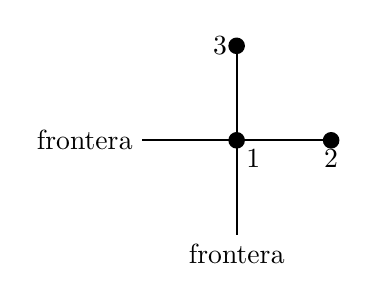
\begin{tikzpicture}[scale=1.2]
		\draw[thick] (-1,0) -- (1,0) (0,-1) -- (0,1);
		\fill (0,0) circle (2.5pt) node[below right] {$1$};
		\fill (1,0) circle (2.5pt) node[below] {$2$};
		\fill (0,1) circle (2.5pt) node[left] {$3$};
		\node[left] at (-1,0) {frontera};
		\node[below] at (0,-1) {frontera};
	\end{tikzpicture}
\end{center}

Sustituyendo cada $(i, j)$ en
\[
4\varphi_{ij} - \varphi_{i-1,j} - \varphi_{i+1,j} - \varphi_{i,j-1} - \varphi_{i,j+1} = 1 :
\]
\begin{align*}
	\text{Nodo } (1,1),\ i = 1,\ j = 1:&\quad 4\underbrace{\varphi_{1,1}}_{\varphi_1} - \underbrace{\varphi_{0,1}}_{0}
	- \underbrace{\varphi_{2,1}}_{\varphi_2} - \underbrace{\varphi_{1,0}}_{0} - \underbrace{\varphi_{1,2}}_{\varphi_3} = 1\\
	\text{Nodo } (2,1),\ i = 2,\ j = 1:&\quad 4\underbrace{\varphi_{2,1}}_{\varphi_2} - \underbrace{\varphi_{1,1}}_{\varphi_1}
	- \underbrace{\varphi_{3,1}}_{0} - \underbrace{\varphi_{2,0}}_{0} - \underbrace{\varphi_{2,2}}_{\varphi_4} = 1\\
	\text{Nodo } (1,2),\ i = 1,\ j = 2:&\quad 4\underbrace{\varphi_{1,2}}_{\varphi_3} - \underbrace{\varphi_{0,2}}_{0}
	- \underbrace{\varphi_{2,2}}_{\varphi_4} - \underbrace{\varphi_{1,1}}_{\varphi_1} - \underbrace{\varphi_{1,3}}_{0} = 1\\
	\text{Nodo } (2,2),\ i = 2,\ j = 2:&\quad 4\underbrace{\varphi_{2,2}}_{\varphi_4} - \underbrace{\varphi_{1,2}}_{\varphi_3}
	- \underbrace{\varphi_{3,2}}_{0} - \underbrace{\varphi_{2,1}}_{\varphi_2} - \underbrace{\varphi_{2,3}}_{0} = 1
\end{align*}

\begin{align*}
	\text{Nodo 1 } (1,1):&\quad 4\varphi_1 - \varphi_2 - \varphi_3 = 1\\
	\text{Nodo 2 } (2,1):&\quad -\varphi_1 + 4\varphi_2 - \varphi_4 = 1\\
	\text{Nodo 3 } (1,2):&\quad -\varphi_1 + 4\varphi_3 - \varphi_4 = 1\\
	\text{Nodo 4 } (2,2):&\quad -\varphi_2 - \varphi_3 + 4\varphi_4 = 1
\end{align*}
La frontera es Dirichlet homogénea

\paso{2}{Sistema y estructura por bloques}
\[
\underbrace{\left(\begin{array}{cc|cc}
		4 & -1 & -1 &  0\\
		-1 &  4 &  0 & -1\\ \hline
		-1 &  0 &  4 & -1\\
		0 & -1 & -1 &  4
	\end{array}\right)}_{\mat{A}}
\begin{pmatrix} \varphi_1\\ \varphi_2\\ \varphi_3\\ \varphi_4 \end{pmatrix}
= \underbrace{\begin{pmatrix} 1\\ 1\\ 1\\ 1 \end{pmatrix}}_{\vect{b}}
\]

Simétrica y pentadiagonal 

Definida positiva 


\inciso{c}{Factor de Cholesky}


\paso{1}{Planteamiento}
Se escribe $\mat{A} = \mat{G}\mat{G}^T$ con todas las incognitas

\[
\begin{pmatrix}
	4 & -1 & -1 &  0\\
	-1 &  4 &  0 & -1\\
	-1 &  0 &  4 & -1\\
	0 & -1 & -1 &  4
\end{pmatrix}
=
\begin{pmatrix}
	g_{11} & 0 & 0 & 0\\
	g_{21} & g_{22} & 0 & 0\\
	g_{31} & g_{32} & g_{33} & 0\\
	g_{41} & g_{42} & g_{43} & g_{44}
\end{pmatrix}
\begin{pmatrix}
	g_{11} & g_{21} & g_{31} & g_{41}\\
	0 & g_{22} & g_{32} & g_{42}\\
	0 & 0 & g_{33} & g_{43}\\
	0 & 0 & 0 & g_{44}
\end{pmatrix}
\]

\begin{align*}
	&\text{Renglón 1:} &
	g_{11}^2 &= a_{11} = 4 & &\Rightarrow\ g_{11} = 2\\
	& & g_{11}g_{21} &= a_{12} = -1 & &\Rightarrow\ g_{21} = -\tfrac12\\
	& & g_{11}g_{31} &= a_{13} = -1 & &\Rightarrow\ g_{31} = -\tfrac12\\
	& & g_{11}g_{41} &= a_{14} = 0 & &\Rightarrow\ g_{41} = 0\\[4pt]
	&\text{Renglón 2:} &
	g_{21}^2 + g_{22}^2 &= a_{22} = 4 & &\Rightarrow\ g_{22} = \sqrt{4 - \tfrac14} = \tfrac{\sqrt{15}}{2}\\
	& & g_{21}g_{31} + g_{22}g_{32} &= a_{23} = 0 & &\Rightarrow\ g_{32} = -\frac{1/4}{\sqrt{15}/2} = -\frac{1}{2\sqrt{15}}\\
	& & g_{21}g_{41} + g_{22}g_{42} &= a_{24} = -1 & &\Rightarrow\ g_{42} = -\frac{1}{\sqrt{15}/2} = -\frac{2}{\sqrt{15}}\\[4pt]
	&\text{Renglón 3:} &
	g_{31}^2 + g_{32}^2 + g_{33}^2 &= a_{33} = 4 & &\Rightarrow\ g_{33} = \sqrt{4 - \tfrac14 - \tfrac{1}{60}} = \sqrt{\tfrac{56}{15}}\\
	& & g_{31}g_{41} + g_{32}g_{42} + g_{33}g_{43} &= a_{34} = -1 & &\Rightarrow\ g_{43} = -\frac{1 + 1/15}{\sqrt{56/15}} = -\frac{8}{\sqrt{210}}\\[4pt]
	&\text{Renglón 4:} &
	g_{41}^2 + g_{42}^2 + g_{43}^2 + g_{44}^2 &= a_{44} = 4 & &\Rightarrow\ g_{44} = \sqrt{4 - \tfrac{4}{15} - \tfrac{32}{105}} = \sqrt{\tfrac{24}{7}}
\end{align*}

\paso{2}{Resultado}
\[
\mat{G} =
\begin{pmatrix}
	2 & 0 & 0 & 0\\[2pt]
	-\tfrac12 & \tfrac{\sqrt{15}}{2} & 0 & 0\\[2pt]
	-\tfrac12 & -\tfrac{1}{2\sqrt{15}} & \sqrt{\tfrac{56}{15}} & 0\\[2pt]
	0 & -\tfrac{2}{\sqrt{15}} & -\tfrac{8}{\sqrt{210}} & \sqrt{\tfrac{24}{7}}
\end{pmatrix},
\qquad
\mat{G}^T =
\begin{pmatrix}
	2 & -\tfrac12 & -\tfrac12 & 0\\[2pt]
	0 & \tfrac{\sqrt{15}}{2} & -\tfrac{1}{2\sqrt{15}} & -\tfrac{2}{\sqrt{15}}\\[2pt]
	0 & 0 & \sqrt{\tfrac{56}{15}} & -\tfrac{8}{\sqrt{210}}\\[2pt]
	0 & 0 & 0 & \sqrt{\tfrac{24}{7}}
\end{pmatrix}
\]


\inciso{d}{Solución del sistema con \texorpdfstring{$\mat{G}$}{G}}

\paso{1}{}
\[
\mat{A}\vect{\varphi} = \vect{b}
\;\Longrightarrow\;
\mat{G}\underbrace{\mat{G}^T\vect{\varphi}}_{\vect{y}} = \vect{b}
\;\Longrightarrow\;
\begin{cases}
	\mat{G}\vect{y} = \vect{b} & \text{(sustitución hacia adelante)}\\
	\mat{G}^T\vect{\varphi} = \vect{y} & \text{(sustitución hacia atrás)}
\end{cases}
\]

\paso{2}{Hacia adelante}
El sistema $\mat{G}\vect{y} = \vect{b}$ es
\[
\begin{pmatrix}
	g_{11} & 0 & 0 & 0\\
	g_{21} & g_{22} & 0 & 0\\
	g_{31} & g_{32} & g_{33} & 0\\
	g_{41} & g_{42} & g_{43} & g_{44}
\end{pmatrix}
\begin{pmatrix} y_1\\ y_2\\ y_3\\ y_4 \end{pmatrix}
=
\begin{pmatrix} b_1\\ b_2\\ b_3\\ b_4 \end{pmatrix}
\quad\Longrightarrow\quad
\begin{aligned}
	g_{11}y_1 &= b_1\\
	g_{21}y_1 + g_{22}y_2 &= b_2\\
	g_{31}y_1 + g_{32}y_2 + g_{33}y_3 &= b_3\\
	g_{41}y_1 + g_{42}y_2 + g_{43}y_3 + g_{44}y_4 &= b_4
\end{aligned}
\]
Como $\mat{G}$ es triangular inferior, se despeja de arriba hacia abajo Con $b_i = 1$ y $g_{41} = 0$:
\begin{align*}
	y_1 &= \frac{b_1}{g_{11}} = \frac{1}{2}\\[8pt]
	y_2 &= \frac{b_2 - g_{21}y_1}{g_{22}}
	= \frac{1 - \left(-\tfrac12\right)\left(\tfrac12\right)}{\tfrac{\sqrt{15}}{2}}
	= \frac{\tfrac54}{\tfrac{\sqrt{15}}{2}} = \frac{\sqrt{15}}{6} \\[8pt]
	y_3 &= \frac{b_3 - g_{31}y_1 - g_{32}y_2}{g_{33}}\\
	&= \frac{1 - \left(-\tfrac12\right)\left(\tfrac12\right) - \left(-\tfrac{1}{2\sqrt{15}}\right)\left(\tfrac{\sqrt{15}}{6}\right)}{\sqrt{\tfrac{56}{15}}}
	= \frac{1 + \tfrac14 + \tfrac{1}{12}}{\sqrt{\tfrac{56}{15}}} = \frac{\tfrac43}{\sqrt{\tfrac{56}{15}}} = \frac{\sqrt{210}}{21} \\[8pt]
	y_4 &= \frac{b_4 - g_{41}y_1 - g_{42}y_2 - g_{43}y_3}{g_{44}}\\
	&= \frac{1 - 0 - \left(-\tfrac{2}{\sqrt{15}}\right)\left(\tfrac{\sqrt{15}}{6}\right) - \left(-\tfrac{8}{\sqrt{210}}\right)\left(\tfrac{\sqrt{210}}{21}\right)}{\sqrt{\tfrac{24}{7}}}
	= \frac{1 + \tfrac13 + \tfrac{8}{21}}{\sqrt{\tfrac{24}{7}}} = \frac{\tfrac{12}{7}}{\sqrt{\tfrac{24}{7}}} = \frac{\sqrt{42}}{7} 
\end{align*}

\paso{3}{Hacia atras}
El sistema $\mat{G}^T\vect{\varphi} = \vect{y}$ es
\[
\begin{pmatrix}
	g_{11} & g_{21} & g_{31} & g_{41}\\
	0 & g_{22} & g_{32} & g_{42}\\
	0 & 0 & g_{33} & g_{43}\\
	0 & 0 & 0 & g_{44}
\end{pmatrix}
\begin{pmatrix} \varphi_1\\ \varphi_2\\ \varphi_3\\ \varphi_4 \end{pmatrix}
=
\begin{pmatrix} y_1\\ y_2\\ y_3\\ y_4 \end{pmatrix}
\quad\Longrightarrow\quad
\begin{aligned}
	g_{11}\varphi_1 + g_{21}\varphi_2 + g_{31}\varphi_3 + g_{41}\varphi_4 &= y_1\\
	g_{22}\varphi_2 + g_{32}\varphi_3 + g_{42}\varphi_4 &= y_2\\
	g_{33}\varphi_3 + g_{43}\varphi_4 &= y_3\\
	g_{44}\varphi_4 &= y_4
\end{aligned}
\]
Ahora $\mat{G}^T$ es triangular superior,se despeja de abajo hacia arriba
\begin{align*}
	\varphi_4 &= \frac{y_4}{g_{44}} = \frac{\tfrac{\sqrt{42}}{7}}{\sqrt{\tfrac{24}{7}}} = \frac12\\[8pt]
	\varphi_3 &= \frac{y_3 - g_{43}\varphi_4}{g_{33}}
	= \frac{\tfrac{\sqrt{210}}{21} - \left(-\tfrac{8}{\sqrt{210}}\right)\left(\tfrac12\right)}{\sqrt{\tfrac{56}{15}}}
	= \frac{\tfrac{\sqrt{210}}{21} + \tfrac{4}{\sqrt{210}}}{\sqrt{\tfrac{56}{15}}} = \frac{\tfrac{\sqrt{210}}{15}}{\sqrt{\tfrac{56}{15}}} = \frac12\\[8pt]
	\varphi_2 &= \frac{y_2 - g_{32}\varphi_3 - g_{42}\varphi_4}{g_{22}}\\
	&= \frac{\tfrac{\sqrt{15}}{6} - \left(-\tfrac{1}{2\sqrt{15}}\right)\left(\tfrac12\right) - \left(-\tfrac{2}{\sqrt{15}}\right)\left(\tfrac12\right)}{\tfrac{\sqrt{15}}{2}}
	= \frac{\tfrac{\sqrt{15}}{6} + \tfrac{1}{4\sqrt{15}} + \tfrac{1}{\sqrt{15}}}{\tfrac{\sqrt{15}}{2}} = \frac{\tfrac{\sqrt{15}}{4}}{\tfrac{\sqrt{15}}{2}} = \frac12\\[8pt]
	\varphi_1 &= \frac{y_1 - g_{21}\varphi_2 - g_{31}\varphi_3 - g_{41}\varphi_4}{g_{11}}\\
	&= \frac{\tfrac12 - \left(-\tfrac12\right)\left(\tfrac12\right) - \left(-\tfrac12\right)\left(\tfrac12\right) - 0}{2}
	= \frac{\tfrac12 + \tfrac14 + \tfrac14}{2} = \frac12
\end{align*}
\resultado{\vect{\varphi} = \left(\tfrac12,\ \tfrac12,\ \tfrac12,\ \tfrac12\right)^T}


\inciso{e}{Malla de \texorpdfstring{$n\times n$}{n x n} nodos interiores}

Una malla de $n\times n$ nodos interiores corresponde a $I = J = n+1$.

\textit{Tamaño de $\mat{A}$}

Hay una incógnita por nodo interior, es decir $n\cdot n = n^2$ incógnitas y $n^2$ ecuaciones:
\resultado{\mat{A}\ \text{es de tamaño}\ n^2\times n^2}

\textit{Ancho de banda}

Con ordenamiento fila por fila, el nodo $k$ se acopla con $k\pm1$ (horizontal) y con $k\pm n$ (vertical). El no cero más lejano de la diagonal es $a_{k,k\pm n}$.

\begin{itemize}
	\item Semiancho de banda: distancia maxima entre la diagonal y un no cero
	\item $\omega_T$ (ancho de banda total): numero de diagonales de la banda, contando la principal y las de ambos lados
	\item $\omega_H$ (ancho de banda medio): la principal mas las diagonales de un solo lado.
\end{itemize}
\resultado{\text{semiancho} = n, \qquad \omega_T = 2n + 1, \qquad \omega_H = n + 1}
Para $n = 2$: $\omega_T = 5$, $\omega_H = 3$ y el no cero más lejano es $a_{13}$.